%\addcontentsline{toc}{chapter}{Development Process}
\chapter{Design}

This chapter describes the design stage of developing Location Sensitive Social Notifier and it also covers in depth the final design that was implemented in the final version of the application.

\section{Overview of architecture}

This section will cover the design of the applications at key stages of development, covering the initial design at the beginning of the project and how it matured to the version that we have today. This section will also cover the future development that will needed to be done to make the application a viable fully fledged application that can be released to the general public.

\subsection{Initial Design}

\subsubsection*{Background}

As the project was done in a iterative and evolutionary style of development there was not much up front planning in the way of initial design. I sketched out a few initial ideas of the block design of the application with all the major parts of the framework including front end, middle tier and database, without any fine details.
The original plan was to use an Oracle APEX backend which would handle all of the REST requests and SQL side of things, but due to licensing and the fact I wanted to learn new technologies this idea fell by the wayside and it was decided to try and use a middle-ware along with a SQL database. \\
\\
It was unclear at the start of the project what platform the application would be developed for, with the choice being between Apple iOS, Google Android or Phone Gapp. So in the early design this left some ambiguity as to how various features and UI design should be implemented. This means in early diagrams the design is very generic and not platform specific.
Theses early sketches were devised from the ideas that had been formulating since I had first envisioned the idea the previous year. The next step was to break the application as a whole and break it down into its functional requirements.\\

\begin{figure}[H]
    \centering
    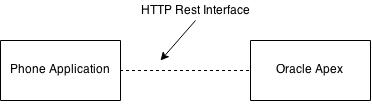
\includegraphics[width=0.5\textwidth]{diagrams/initialblockdiagram}
    \caption{Original design of the application}
    \label{fig:apex_block_diagram_image}
\end{figure} 

\subsubsection*{Functionality}

%ALISON READ THIS.

Assessing the functional requirements required breaking down the concept into its core components. Most noticeably posting, viewing and being notified about tags were the core functionality for the application without theses features the application could not achieve the goals set out in the original specification thus undermining the usefulness of the finished application.\\
\\
Viewing a message that is left in the application is a core part of the functionality that is required by the application, it should be very easy and uncomplicated for the user to view a tag that has been left by there friends. The application's overall success will most possibly rest on the speed of viewing a message and quickly being able to leave feedback on the tag that has been left. The UI should be easy to intemperate with the minimal UI on the screen to ensure that there is no confusion in the message trying to be convey, a simple and minimal UI also gives the application an attractive aesthetic that should mean that users are attracted to using the application. It should be easy for the user to decide if the tag is publicly available or limited to friends to ensure the flexibility of the application.\\
\\
An equally important feature that makes the application is the posting of messages, without the ability to post a message the application is a void concept and generally to view messages there needs to be the ability to post messages. Again the key aim of the application is to make it easy to leave messages without any extra complexity that might discourage the user from leaving a message. The UI should be as minimal as possible while portraying the intent of the screen in a simple and straight forward way most, some clever UI design should help draw the interest into the page and enable the user understand what is happening, the use of a map fragment on this page to show where the user is when they post there message is a good way to draw attention into the posting of a message. The user should be able to enter a message of a reasonable length into the fields within the application.\\
\\
The final core functionality that is integral to get the application to work as desired is the notification portion which notifies the user of the tags that are near by to the user, this should run with no input from the user and should quickly and efficiently provide the user information about the nearby tag, when the user interacts with the notification then they should be able to quickly and effectively navigate to the view message page they will not have to go into the application its self to select this but the notification will automatically take the user to the view message screen for them to interpret what the message is.\\
\\
More minor functionality is dealing with friends within the application so adding the users friends so that they can interact with them within the application, adding friends to there account should be straightforward with a search that enables them to find and add them to there account, this should also not be a cluttered page with the bare minimum UI elements to get the job done correctly as this should minimise the confusion from using the application and means it should be more likely that users user the application and recommend it onto the friends to actually use it. Continuation of the friends theme is that it should be very easy for users to add viability to messages for there friends to view it, giving a user viability should mean that they will get notified of the message when they are close by to it.\\
\\
The application will also require having some operations for dealing with authentication with the server so it is essential for the application to have screens to register and login theses screens should be as simple as possible and still get the job done only asking the true essentials to get the job done. With clear and simple forms that will not lead to confusion and frustration that would lead to them being put off using the application, keeping the forms simple should also improve security as its less fields to protect from attack and thus being compromised by an potential malicious user.\\

\subsubsection*{UI mock-ups}

Once the application had been broken down into the various functional areas I started to do some rough user interface layouts on paper. Once they were to a satisfactory level they were converted into digital mock-ups using Balsamiq which created the figures \ref{fig:application_home_page_image}, \ref{fig:add_friend_activity_image}, \ref{fig:add_tag_activity_image}, \ref{fig:viewing_message_image}, \ref{fig:giving_friends_visability_image}, \ref{fig:login_activity_image}, \ref{fig:registration_activity_image} and \ref{fig:notification_image}. \\
\\
The UI design takes some inspiration from other phone applications, in particular Snap Chat with the way of quickly sharing messages and Facebook with the quickly accessible stacked menus. The main reason I took inspiration from Snap Chat is because their application is very quick to use and post messages and the general concept of Lo Se Sono is almost the same bar and locations are used rather than pictures and there is no set timeout on the tags.\\
\\
At the time of creating the mock ups it was not clear for which platform the application was going to be implemented, so the designs have remained very generic without being OS specific.\\
\\
These UI mock-ups were used to create the final application. The designs may have been slightly modified between the original design and the final implementation within the application.\\
\\
Figure \ref{fig:application_home_page_image} is the design for the main page of the application and where the users arrive when the application launches, so it is of utmost importance that this page is easy to navigate and informative to the user. The UI has been intentionally designed to show the tags that are most relevant to the user at the time they have opened the application, showing the tags in their immediate vicinity. These can be either the user's own tags or their friends who have left them there.\\

\begin{figure}[H]
    \centering
    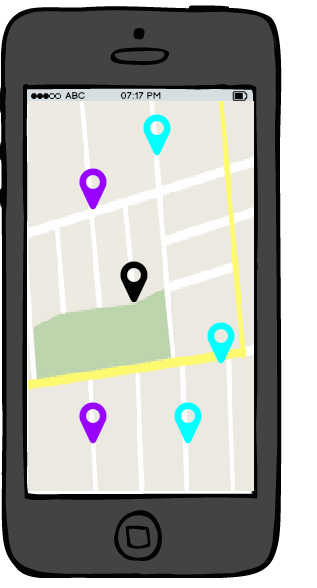
\includegraphics[width=0.25\textwidth]{uimockups/homepage}
    \caption{Application home page}
    \label{fig:application_home_page_image}
\end{figure}

\noindent
In figure \ref{fig:add_tag_activity_image} we are showing the initial design for adding a tag to the map. The key idea is to make it quick and easy to add a tag to the map and make it quickly accessible to the user's friends so they can be promptly notified about the tag their friend has added.\\

\begin{figure}[H]
    \centering
    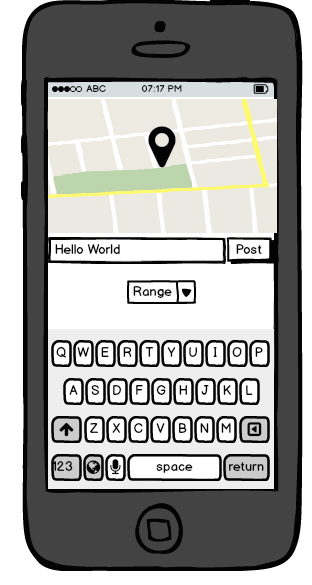
\includegraphics[width=0.25\textwidth]{uimockups/addtag}
    \caption{Adding a tag activity}
    \label{fig:add_tag_activity_image}
\end{figure}

\noindent
Pictured in figure \ref{fig:giving_friends_visability_image} is the screen that enables user's friends to view a message that has been left. It should be relatively straight forward and easy to interpret. The design has changed ever so slightly in the final implementation to try and make it fit in better with the Android design principles.\\

\begin{figure}[H]
    \centering
    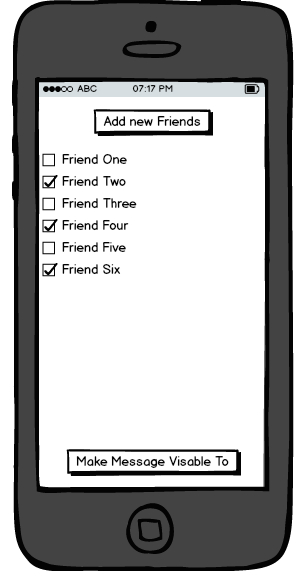
\includegraphics[width=0.25\textwidth]{uimockups/friendsvisability}
    \caption{Giving friends ability to view message}
    \label{fig:giving_friends_visability_image}
\end{figure} 

\noindent
This is the UI in figure \ref{fig:add_friend_activity_image}. To add a new user to the user's friends list it gives the user the ability to search for their friends using their names. In the final version of the application the search functionality remains unfinished within the UI, but was partially completed within the server side application. When this functionality is implemented it should make it very easy for the user to add new friends within the application, thus expanding the audience of the application.\\

%Alison got to here.

\begin{figure}[H]
    \centering
    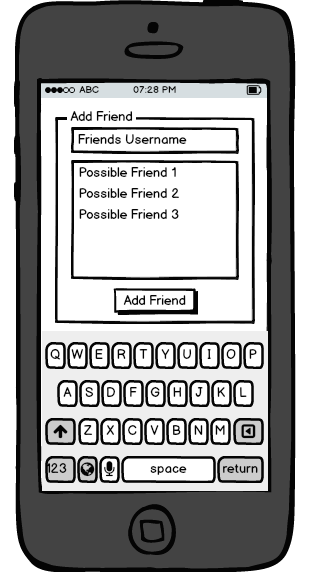
\includegraphics[width=0.25\textwidth]{uimockups/addfriend}
    \caption{Adding Friend activity}
    \label{fig:add_friend_activity_image}
\end{figure} 

\noindent
In this figure \ref{fig:viewing_message_image} we are show the viewing of a message, this is the screen that has changed the most from the original UI mock ups, where the icons and location of the voting section has been moved to be above the commenting area, there is also now a fixed area at the bottom for adding a comment along with each comment section now including there own voting sections, but again the changes to the initial designs intentionally have been very minor.\\

\begin{figure}[H]
    \centering
    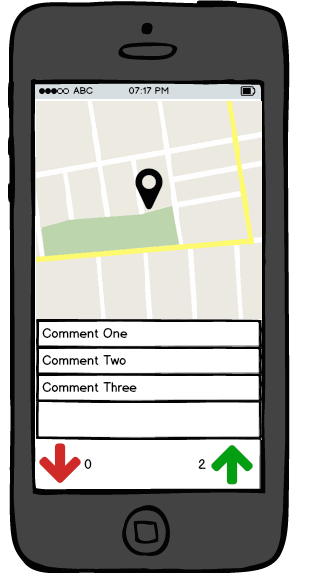
\includegraphics[width=0.25\textwidth]{uimockups/viewmessage}
    \caption{Viewing a message}
    \label{fig:viewing_message_image}
\end{figure} 

\noindent
The image below in figure \ref{fig:login_activity_image} shows the login screen for the application, this was intentionally kept simplistic to ensure that it is easy for the user to intemperate and should make it fairly secure against attacks as there are less fields to attack.\\

\begin{figure}[H]
    \centering
    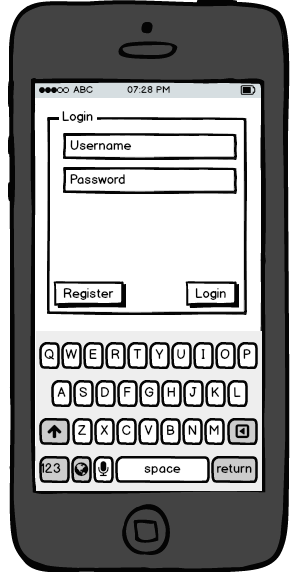
\includegraphics[width=0.25\textwidth]{uimockups/login}
    \caption{Login Activity for the application}
    \label{fig:login_activity_image}
\end{figure} 

\noindent
Screenshot pictured in figure \ref{fig:registration_activity_image} describes the registration page within the application that enables the user to register to use the application, again it has been kept simple to avoid confuse and ensure that the user can navigate it easily, this should easy annoyance when people are using the application for the first time.\\

\begin{figure}[H]
    \centering
    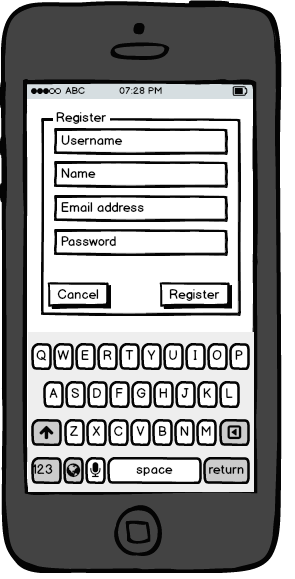
\includegraphics[width=0.25\textwidth]{uimockups/register}
    \caption{This is the activity for registering to use the application}
    \label{fig:registration_activity_image}
\end{figure} 

\noindent
This screenshot in figure \ref{fig:notification_image} is an example notification for the application, in the final application this does not look anything like this due to the fact we are using the Google Android notification API and notifications do not appear in this way.\\

\begin{figure}[H]
    \centering
    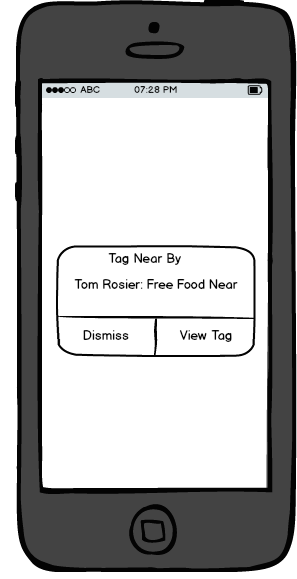
\includegraphics[width=0.25\textwidth]{uimockups/notification}
    \caption{Notification that there is a tag near by}
    \label{fig:notification_image}
\end{figure} 

\noindent
Theses designs were used as reference to build the applications UI for the final design, they have intentionally kept similar to the original mock-ups as it was felt that the designs would be easy for users to interpret and a good starting point.\\

\subsection{Final Implementation}

As the project was developed in a eXtream programing style there was not much design done up front, the major design that was done up front was a list of the main functionality within the application and the final implementation of those features were done in an iterative form. There was a very initial block diagram done showing the different main sections of the application this is showing in figure \ref{fig:initial_diagram_image} this is the basic design of the application without any of the specifics e.g not detailing the libraries that have been used to implement the full application.\\

\begin{figure}[H]
    \centering
    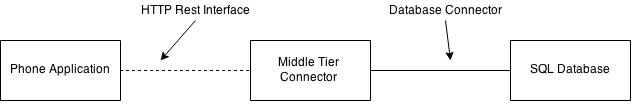
\includegraphics[width=\textwidth]{diagrams/blockdiagram}
    \caption{Very simple block diagram from the start of development}
    \label{fig:initial_diagram_image}
\end{figure} 

\noindent
The final implementation started with spike work into different frameworks that could be used for the development of the project, we started with the Phone side of the application where there was research into weather to use Phone Gapp or to go for a native application the reasoning and decision to use an exclusively Google Android are covered in section "\ref{sec:android_choice_of_tech} Choice of technologies".\\
\\
Next the focus moved onto the server side application, the focus for the choice of server side environment was focused on looking at cutting edge but also fairly mature server side platforms, the choice was between Node.js with express, Node.js with HAPI.js, Node.js with StrongLoop, Python Flask or Java TomCat please refer to "\ref{sec:node_choice_of_tech} Choice of technologies" for more in detail discussion about the rational between the choice of server side frameworks.\\
\\
Finally the decision turned to how the data would be stored within the application the first decision was between a SQL or NOSQL solution, after some consideration it was considered that even though NOSQL is a interesting new area it was decided to stick with the skills already learn as taking on to many new frameworks could compromise the success of the project. The final decision was to decide between what type of SQL engine to use to hold and process the data within the application the decision was between PostgresSQL, My-SQL and SQLite. The pro's and con's are covered in detail in section "\ref{sec:database_choice_of_tech} Choice of technologies".\\
\\
The diagram in figure \ref{fig:final_block_diagram_image} shows the finished architecture with the joins between each different technology that is needed to make the application work correctly and as desired in the way decided within the functional requirements. It is fairly obvious from the diagram that the application requires a lot of 3rd party libraries to work as intended heavily relying on the Google Maps API, Android Asynchronous HTTP Client API, HAPI.js \& Sequelize to provide the major components within the project.\\

\begin{figure}[H]
    \centering
    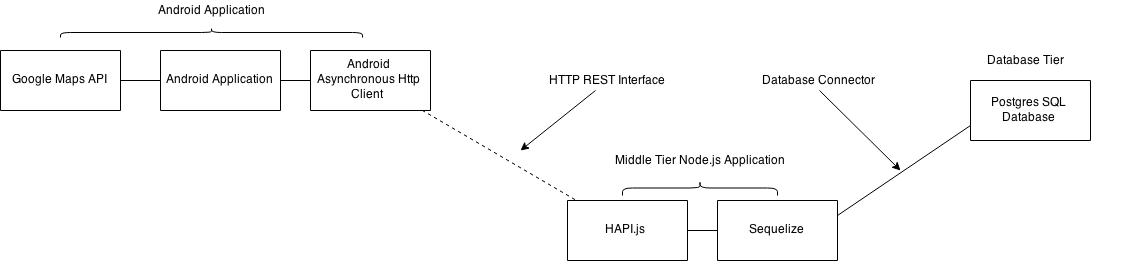
\includegraphics[width=\textwidth]{diagrams/finalblockdiagram}
    \caption{Very simple block diagram of the final architecture}
    \label{fig:final_block_diagram_image}
\end{figure}

\noindent
Standing on the shoulders of giants springs to mind as it would not be possible without all of theses 3rd party libraries for the application work in a usable and robust manner, even with the use of all these 3rd party libraries there is still a fair bit of custom code to act as a aggregate all the various parts of the functionality within the project together. The core functionally of the application is complete, but I would currently classify the application as a proof of concept due to the fact the robustness of the application and stability are currently questionable how these issues will be overcome in the future will be covered in section \ref{sec:development_future_dev}.\\

\subsection{Future Development}
\label{sec:development_future_dev}

{TODO}

%Power considerations

%Scalability for different screen resolutions.

%Robust error handling.


\section{Client Side}

{TODO}

\subsection{Android Application}

{TODO}

\subsubsection*{Choice of Technologies}
\label{sec:android_choice_of_tech}

The spike work / research that was carried out in the design stage started out by reading about the development experiences of various teams Phone Gapp vs Native to develop there various phone application and the reviews that I got seemed to be very mixed they ranged from saying to avoid or this is the best thing ever, with no clear way to move forward it the next stage was to research the API's that would be essential to the application working this being the Mapping API's and the GPS location. It quickly came apparent although Phone Gapp its fairly mature it could not compare to the libraries that were offered by the native solution.\\
\\
One of the benefits of using Phone Gapp over native is that it uses standard web technologies for example HTML, JavaScript \& CSS which I as the developer already knew fairly well and would not need to learn a new language to work on the application but this would still require learning a new framework to work on the application. Another benefit of using Phone Gapp is that the application will run on a multitude of devices from Apple iOS, Google Android and Microsoft Windows Phone where as choosing to go native means that application will only work on the framework and device it is programmed for.\\
\\
One of the major downsides of using Phone Gapp is that if there is not a library that exists for a given problem within the application then the developer is required to write in native code a library to couple the Phone Gapp application to the function provided by the phone. Due to this it was decided it would be best to just develop the application in native code as it eliminates theses coupling issues if they do arise. Along with the extra performance given by running within the native framework and not having another interpretive layer between the user and the phones hardware gives the developer and ultimately a better experience with the application.\\
\\



\subsubsection*{Initial Design}

{TODO}

\subsubsection*{Application Structure}

{TODO}

\subsubsection*{Caveats}

{TODO}

% Talk about first time using android.



\section{Server Side}

{TODO}

\subsection{Middle Tier}

{TODO}

\subsubsection*{Choice of Technologies}
\label{sec:node_choice_of_tech}

{TODO}

\subsubsection*{Rest interface}

{TODO}

\begin{figure}[H]
    \centering
    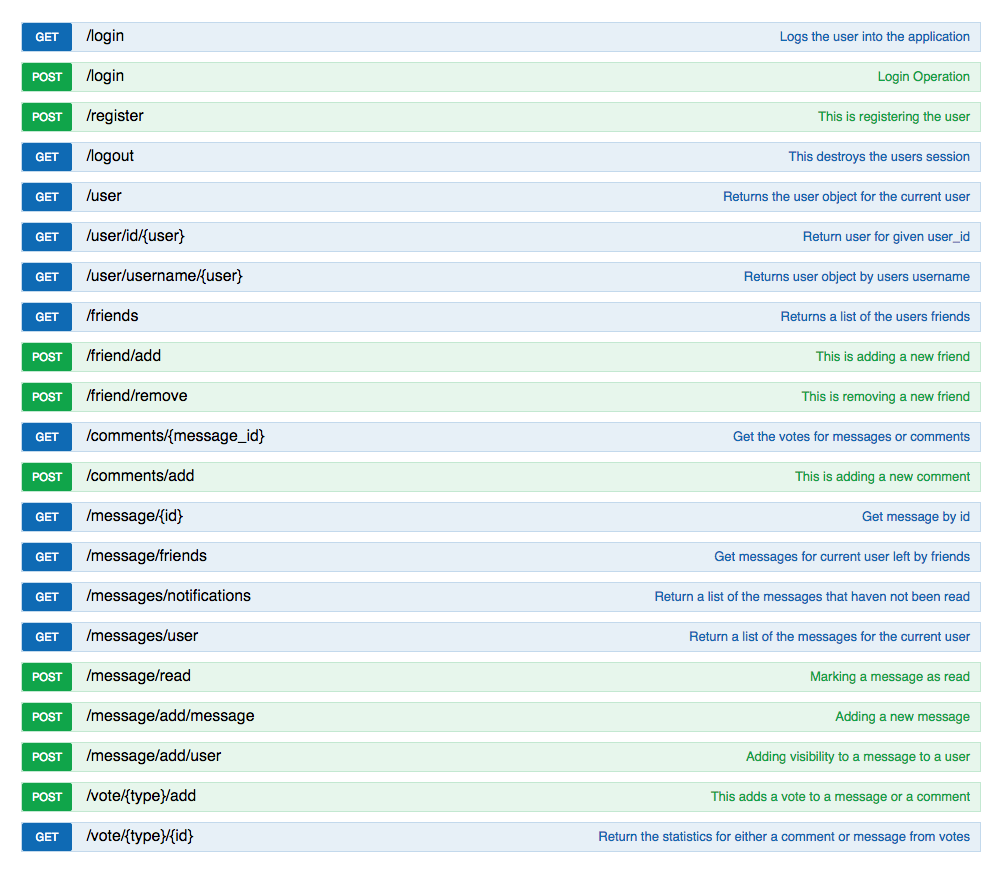
\includegraphics[width=\textwidth]{diagrams/restinterface}
    \caption{These are the endpoints for the REST API}
    \label{fig:rest_pai_diagram_image}
\end{figure} 
\noindent

\subsubsection*{Structure of application}

{TODO}

\subsubsection*{Authentication}

{TODO}

\subsection{Database level}

{TODO}

\subsubsection*{Choice of Technologies}
\label{sec:database_choice_of_tech}

{TODO}

\subsubsection*{Database structure}

{TODO}

\begin{figure}[H]
    \centering
    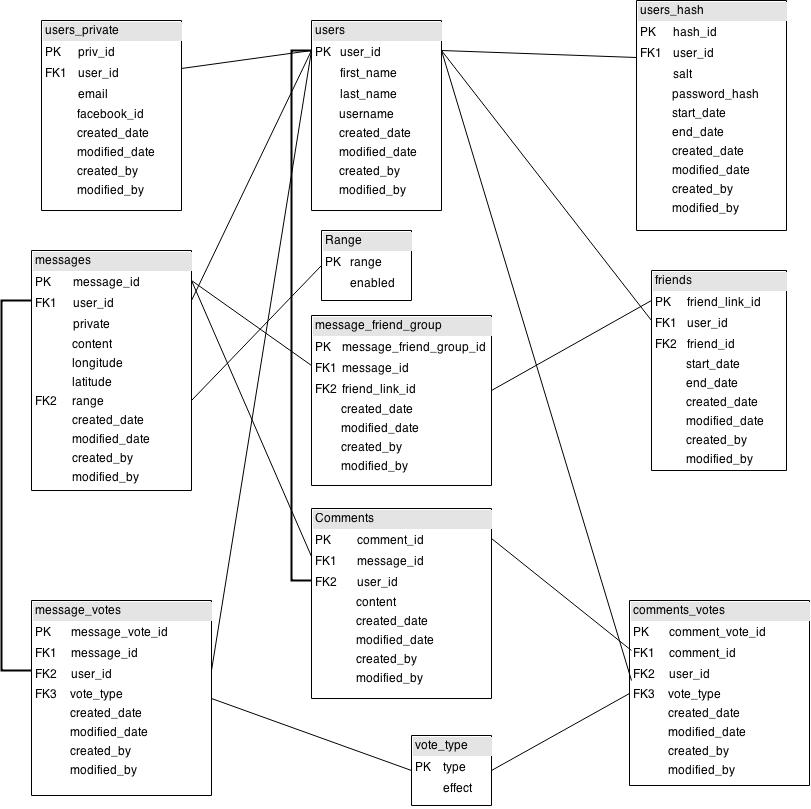
\includegraphics[width=\textwidth]{diagrams/database}
    \caption{This is the database design for the application}
    \label{fig:diagram_database_image}
\end{figure} 
\noindent

\subsubsection*{Alterations}

{TODO}

\subsubsection*{Protecting secrets}

{TODO}